\documentclass[11pt,a4paper]{article}
\usepackage[utf8]{inputenc}
\usepackage[T1]{fontenc}
\usepackage{lmodern}
\usepackage[a4paper,margin=2cm,bottom=2.5cm]{geometry}
\usepackage{graphicx}
\usepackage[export]{adjustbox}
\usepackage{float}
\usepackage{xcolor}
\usepackage{listings}
\usepackage{upquote}
\usepackage{enumitem}
\usepackage{fancyhdr}
\usepackage{xurl}
\usepackage[colorlinks=true,linkcolor=kulblue,urlcolor=kulblue]{hyperref}

\definecolor{kulblue}{RGB}{29, 141, 176}
\definecolor{codegreen}{rgb}{0,0.5,0}
\definecolor{codegray}{rgb}{0.5,0.5,0.5}
\definecolor{codepurple}{rgb}{0.58,0,0.82}
\definecolor{backcolour}{rgb}{0.95,0.95,0.97}

\lstdefinelanguage{CUDA}[]{C++}{
  morekeywords={__global__,__device__,__host__,__shared__,dim3,
    threadIdx,blockIdx,blockDim,gridDim,warpSize,
    cudaMallocManaged,cudaMalloc,cudaMemcpy,cudaFree,cudaDeviceSynchronize,
    cudaMemcpyHostToDevice,cudaMemcpyDeviceToHost,cudaGetLastError,cudaGetErrorString,
    cudaEvent_t,cudaEventCreate,cudaEventRecord,cudaEventSynchronize,cudaEventElapsedTime},
}

\lstdefinestyle{gca}{
  backgroundcolor=\color{backcolour},
  commentstyle=\color{codegreen},
  keywordstyle=\color{magenta}\bfseries,
  stringstyle=\color{codepurple},
  numberstyle=\tiny\color{codegray},
  basicstyle=\ttfamily\scriptsize,
  columns=fullflexible,
  breaklines=true,
  breakatwhitespace=false,
  postbreak=\mbox{\textcolor{codegray}{$\hookrightarrow$}\space},
  keepspaces=true,
  numbers=left,
  numbersep=6pt,
  showstringspaces=false,
  upquote=true,
  tabsize=4,
  frame=single,
  rulecolor=\color{backcolour},
  xleftmargin=1.5em,
  framexleftmargin=1.5em,
  literate={—}{{---}}1 {×}{{$\times$}}1 {’}{{'}}1,
}
\lstset{style=gca}

\setlength{\parindent}{0pt}
\setlength{\parskip}{0.6em}

\usepackage{subfiles}

\newcommand{\headtitle}{GCA}
\newcommand{\headdate}{}
\newcommand{\gcapart}[2]{%
  \clearpage
  \renewcommand{\headtitle}{GCA -- #1}\renewcommand{\headdate}{#2}%
  \phantomsection\addcontentsline{toc}{part}{#1}\part*{#1}}
\newcommand{\session}[2]{%
  \ifSubfilesClassLoaded{%
    \renewcommand{\headtitle}{GCA -- Session #1}\renewcommand{\headdate}{#2}%
    \title{\textbf{GCA -- Session #1}\\[2mm]\large Geavanceerde Computerarchitectuur}%
    \date{#2 \quad (academic year 2026/2027)}%
    \maketitle\thispagestyle{fancy}\tableofcontents\newpage
  }{\gcapart{Session #1}{#2}}}

\pagestyle{fancy}
\fancyhf{}
\fancyhead[L]{\small \headtitle}
\fancyhead[R]{\small Geavanceerde Computerarchitectuur}
\fancyfoot[L]{\small \headdate}
\fancyfoot[C]{\small \thepage}
\fancyfoot[R]{\IfFileExists{figures/KULEUVEN_GENT_RGB_LOGO.png}{
\includegraphics[width=2cm]{figures/KULEUVEN_GENT_RGB_LOGO.png}}{}}
\renewcommand{\headrulewidth}{0.4pt}

\title{\textbf{GCA}\\[2mm]\large Geavanceerde Computerarchitectuur}
\author{Joris Putteneers\\\href{mailto:joris.putteneers@kuleuven.be}{\texttt{joris.putteneers@kuleuven.be}}}
\date{academic year 2026/2027}

\begin{document}
\maketitle
\thispagestyle{fancy}
\tableofcontents
\newpage

%=====================================================================
\section{Introduction}

\subsection{Goals, learning outcomes, and expectations}

The goal of this course is to introduce students to the fundamentals of general purpose GPU programming. We shall dive into the concepts of parallel multi-thread processing, learning how to leverage the large number of GPU cores and how to efficiently use the device's memory. Among others, concepts such as atomic operation, synchronous multi-threading, and dynamic parallelism are explored during the course. In addition to guided exercises, the students will partake in a short project, tackling a research or programming challenge of their liking using the newly acquired knowledge. By the end, the students are foreseen to have the necessary understanding of GPUs and parallel programming that will allow them to utilize GPUs in their future work. Throughout the course NVIDIA GPUs and C++ are employed (CUDA API).
\begin{figure}[H]
\centering
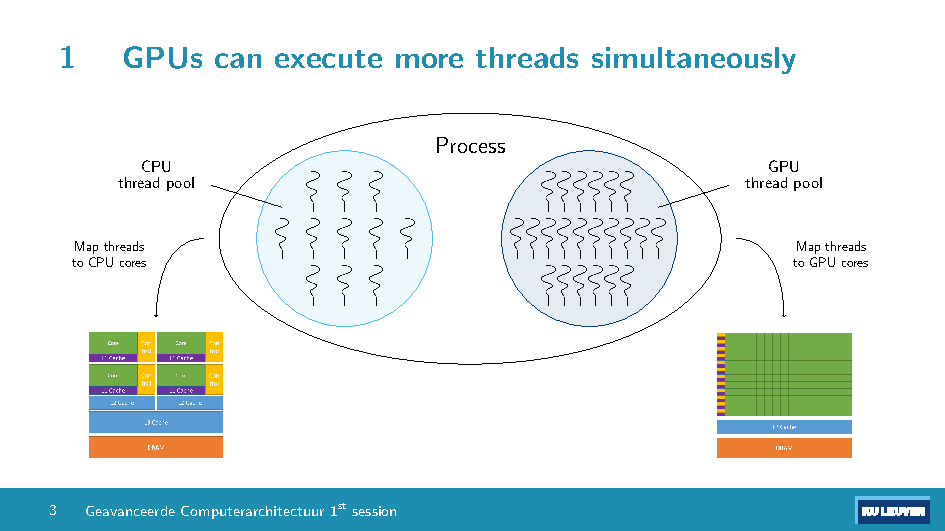
\includegraphics[width=0.72\linewidth, trim=0 20pt 0 0, clip, frame]{figures/session_1_figures/slide-04.pdf}
\caption{GPUs can execute more threads simultaneously than CPUs.}
\end{figure}
\begin{figure}[H]
\centering
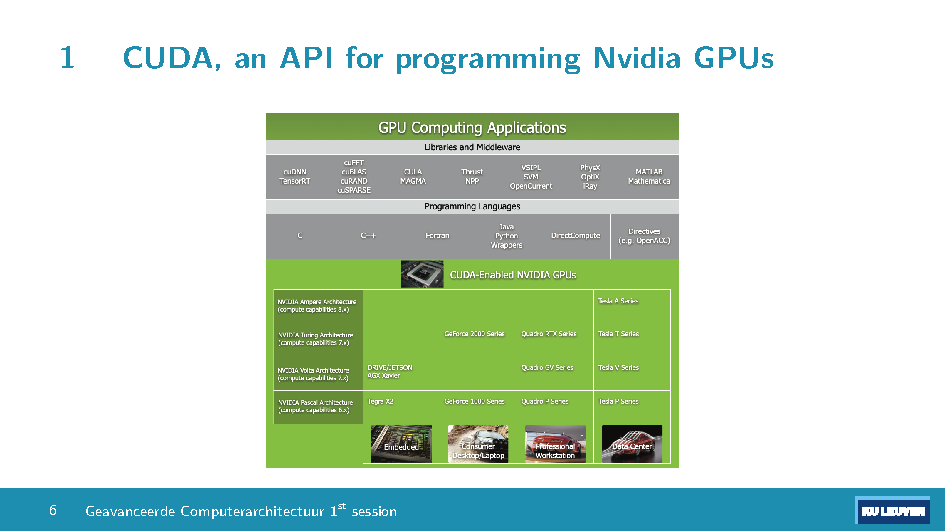
\includegraphics[width=0.72\linewidth, trim=0 20pt 0 0, clip, frame]{figures/session_1_figures/slide-09.pdf}
\caption{CUDA, an API for programming NVIDIA GPUs.}
\end{figure}

\subsection{Lab sessions}

The below sections outline the six guided lab sessions (each 3h).

\textbf{Organization} --- 12 sessions in total:
\begin{itemize}[nosep]
  \item 5 lab sessions
  \item 7 project sessions (6 project, 1 presentations)
\end{itemize}

\subsection{Responsibilities and evaluation}

\begin{minipage}[t]{0.48\linewidth}
\textbf{Lab sessions: 50\%}
\begin{itemize}[nosep]
  \item 5 single-page reports, one per lab session
\end{itemize}
\end{minipage}\hfill
\begin{minipage}[t]{0.48\linewidth}
\textbf{Project: 50\%}
\begin{itemize}[nosep]
  \item Project report
  \item Project presentation
  \item Code release
\end{itemize}
\end{minipage}

%=====================================================================
\section{Project}

\subsection{Goal and organization}
\begin{itemize}
  \item The goal of the project is to tackle a computational challenge using the GPU.
  \item This should be something that aligns with your interests -- to support your thesis or another lab; to implement something for a hobby / private project; to boost your portfolio and get a better job.
  \item We will allocate 5 lab sessions to development and 1 session to the presentations.
\end{itemize}

\subsection{Implementation}
\begin{itemize}
  \item Use the concepts we have gotten acquainted with so far and feel free to explore other paradigms. You can use another programming language and also build on another library -- keep in mind that you should still understand and describe the intricacies of the implementation.
\end{itemize}

\subsection{Some topic examples}
In case you don't know where to start, here are a few biased examples:
\begin{itemize}
  \item An RF \textbf{ray tracer} to determine how Wi-Fi waves propagate in (and outside of) your kot.
  \item An \textbf{optimization algorithm} to determine where to put the Wi-Fi router for optimal coverage (considering either only yourself or all inhabitants).
  \item \textbf{Data compression} on an edge device that collects sensor samples and analyzes/compresses/transforms these in order to send the information over a low-throughput link.
  \item Real-time \textbf{statistical analysis} of a video stream.
\end{itemize}

\subsection{Grading -- guidelines based on thesis evaluation matrix}

\textbf{Implementation}
\begin{itemize}[nosep]
  \item The implementation works, while clearly addressing the tackled problem
  \item Includes the concepts introduced in the lab or sufficiently motivates other approaches
\end{itemize}

\textbf{Report} (no min/max length -- try to be concise)
\begin{itemize}[nosep]
  \item Clearly describes the problem and motivates the usage of the GPU
  \item Introduces the implementation and methods in detail (includes references to the repository or code listings)
  \item Highlights the shortcomings and possible improvements
\end{itemize}

\textbf{Presentation} (up to 10 min + 10 min for Q\&A)
\begin{itemize}[nosep]
  \item Clearly describes the problem and motivates the usage of the GPU
  \item Provides a high-level overview of the implementation
  \item Highlights the shortcomings and possible improvements
\end{itemize}

\subsection{Important dates}
Please submit the reports on time, so we can close off the lab on the day of the presentations (focus on the thesis / exams afterwards).

%=====================================================================
\section{Where to run?}
\begin{figure}[H]
\centering
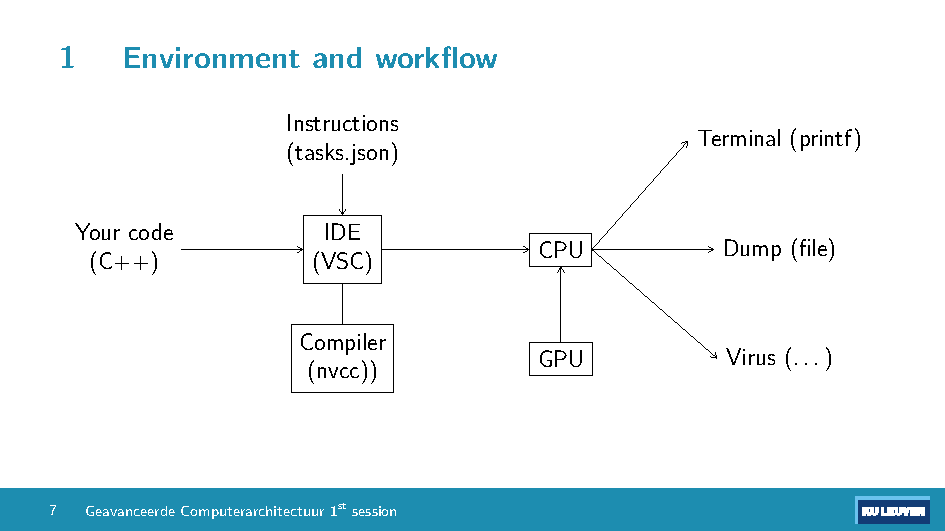
\includegraphics[width=0.72\linewidth, trim=0 20pt 0 0, clip, frame]{figures/session_1_figures/slide-10.pdf}
\caption{Environment and workflow.}
\end{figure}

\subsection{On the lab PCs (no GPU of your own)}
\begin{enumerate}
  \item Use a desktop with a grey/silver front: these have an NVIDIA GPU (from next week).

  \begin{tabular}{@{}ll}
    GPU: & NVIDIA GeForce GT 730\\
    Compute capability: & 3.5\\
    Memory: & 1024 MB\\
    SMs: & 2 (192 cores per SM, 384 cores total)
  \end{tabular}
  \item Boot into Linux (not Windows).
  \item Log in:

  \begin{tabular}{@{}ll}
    user: & \texttt{student}\\
    password: & \texttt{studentXX} \quad (XX = the PC number)
  \end{tabular}

  Admin password (only if something needs to be changed): ask the teacher.
  \item Test:
\begin{lstlisting}[language=bash,numbers=none]
nvcc -arch=sm_35 -o hello hello.cu && ./hello
\end{lstlisting}
\end{enumerate}

\subsection{On your own laptop: Windows with WSL}
\begin{enumerate}
  \item Windows: check the laptop has an NVIDIA GPU, then install the latest NVIDIA driver from nvidia.com. Do \textbf{not} install any Linux driver inside WSL.
  \item PowerShell (admin):
\begin{lstlisting}[language=bash,numbers=none]
wsl --install
\end{lstlisting}
  Restart, open Ubuntu, create a user.
  \item Ubuntu:
\begin{lstlisting}[language=bash,numbers=none]
nvidia-smi
sudo apt update && sudo apt install -y build-essential
wget https://developer.download.nvidia.com/compute/cuda/repos/wsl-ubuntu/x86_64/cuda-keyring_1.1-1_all.deb
sudo dpkg -i cuda-keyring_1.1-1_all.deb
sudo apt update && sudo apt install -y cuda-toolkit
echo 'export PATH=/usr/local/cuda/bin:$PATH' >> ~/.bashrc && source ~/.bashrc
\end{lstlisting}
  \texttt{nvidia-smi} must show the GPU.\\
  GTX 10-series (Pascal) laptops: use \texttt{cuda-toolkit-12-9} instead of \texttt{cuda-toolkit}.
  \item VS Code: install on Windows + the ``WSL'' extension. Then in Ubuntu:
\begin{lstlisting}[language=bash,numbers=none]
mkdir ~/gca && cd ~/gca && code .
\end{lstlisting}
  Put the course \texttt{tasks.json} in \texttt{\textasciitilde/gca/.vscode/}
  \item Test:
\begin{lstlisting}[language=bash,numbers=none]
nvcc -o hello hello.cu && ./hello
\end{lstlisting}
\end{enumerate}

\subsection{On your own laptop: Linux (Ubuntu 24.04)}
\begin{enumerate}
  \item Driver:
\begin{lstlisting}[language=bash,numbers=none]
sudo ubuntu-drivers install
sudo reboot
nvidia-smi
\end{lstlisting}
  \texttt{nvidia-smi} must show the GPU. Top right it shows ``CUDA Version'': the newest CUDA this driver supports.
  \item Toolkit:
\begin{lstlisting}[language=bash,numbers=none]
sudo apt update && sudo apt install -y build-essential
wget https://developer.download.nvidia.com/compute/cuda/repos/ubuntu2404/x86_64/cuda-keyring_1.1-1_all.deb
sudo dpkg -i cuda-keyring_1.1-1_all.deb
sudo apt update && sudo apt install -y cuda-toolkit
echo 'export PATH=/usr/local/cuda/bin:$PATH' >> ~/.bashrc && source ~/.bashrc
\end{lstlisting}
  \begin{itemize}[nosep]
    \item Install only \texttt{cuda-toolkit} (not \texttt{cuda}: that also installs a second driver).
    \item The toolkit version (\texttt{nvcc --version}) must not be newer than the ``CUDA Version'' in \texttt{nvidia-smi}. If it is, or on GTX 10-series (Pascal) GPUs: use \texttt{cuda-toolkit-12-9} instead.
    \item Ubuntu 22.04: replace \texttt{ubuntu2404} with \texttt{ubuntu2204} in the \texttt{wget} line.
  \end{itemize}
  Simplest alternative (older CUDA 12.0, no PATH step needed):
\begin{lstlisting}[language=bash,numbers=none]
sudo apt install -y nvidia-cuda-toolkit
\end{lstlisting}
  \item VS Code:
\begin{lstlisting}[language=bash,numbers=none]
sudo snap install code --classic
mkdir ~/gca && cd ~/gca && code .
\end{lstlisting}
  Install the C/C++ extension. Put the course \texttt{tasks.json} in \texttt{\textasciitilde/gca/.vscode/}
  \item Test:
\begin{lstlisting}[language=bash,numbers=none]
nvcc -o hello hello.cu && ./hello
\end{lstlisting}
\end{enumerate}

\subfile{session_1}
\subfile{session_2}
\gcapart{Cheat sheet}{}
This section lists several functions, definitions, etc., handy for the GCA lab. It is a living document, where updates are added according to the lab sessions and feedback from the students. Thanks for pointing things out.

\textbf{GPU memory allocation}
\begin{lstlisting}[language=CUDA,numbers=none]
float* d_A;
cudaMalloc(&d_A, size);
\end{lstlisting}

\textbf{Memory migration to / from GPU}
\begin{lstlisting}[language=CUDA,numbers=none]
float* h_A = (float*)malloc(size);
cudaMemcpy(d_A, h_A, size, cudaMemcpyHostToDevice);
cudaMemcpy(h_A, d_A, size, cudaMemcpyDeviceToHost);
\end{lstlisting}

\textbf{Kernel invocation (100 blocks, with 80 threads each)}
\begin{lstlisting}[language=CUDA,numbers=none]
foo<<<100, 80>>>(d_A);
\end{lstlisting}

\textbf{Thread indexing}
\begin{lstlisting}[language=CUDA,numbers=none]
int i = threadIdx.x;
\end{lstlisting}

\textbf{Setting to global scope (invoked by CPU or GPU)}
\begin{lstlisting}[language=CUDA,numbers=none]
__global__ void foo(d_A){...}
\end{lstlisting}

\textbf{Setting to GPU scope (invoked by GPU)}
\begin{lstlisting}[language=CUDA,numbers=none]
__device__ float foo(d_A){...}
\end{lstlisting}

\textbf{Timing (CPU)}
\begin{lstlisting}[language=CUDA,numbers=none]
#include <chrono>
const auto start = std::chrono::steady_clock::now();
...
const auto end = std::chrono::steady_clock::now();
const std::chrono::duration<double> elapsed_seconds{end - start};
\end{lstlisting}

\textbf{Timing (GPU)}
\begin{lstlisting}[language=CUDA,numbers=none]
cudaEvent_t start, stop;
cudaEventCreate(&start);
cudaEventCreate(&stop);
cudaEventRecord(start);
...
cudaEventSynchronize();
cudaEventRecord(stop);
float milliseconds;
cudaEventElapsedTime(&milliseconds, start_cuda, stop_cuda);
\end{lstlisting}


\end{document}
